\chapter{Implementatie}

\section{Checkin}

Als de gebruiker het lab binnen loopt, moet hij eerst inchecken. Om dat mogelijk te maken is een apart pagina gemaakt. Deze pagina is in 
Figuur \ref{fig:checkinoutview} te zien. Het bestaat uit 3 hoofdcomponenten: het welkomsbericht, de checkin knoppen en de checkout tabel.

\begin{figure}[Hh]
	\centering
	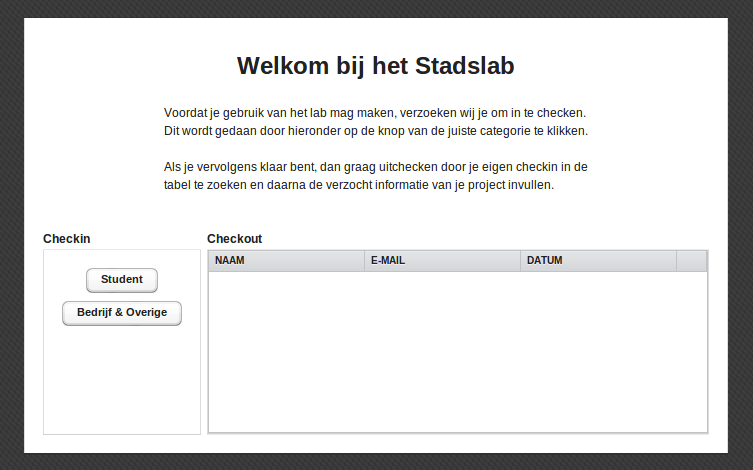
\includegraphics[width=\textwidth]{Images/checkinoutview2.png}
	\caption{Venster waar kan worden ingecheckt en uitgecheckt}
	\label{fig:checkinoutview}
\end{figure}

Het welkomsbericht bestaat uit een korte stuk tekst waarin uitgelegd wordt wat de bedoeling van deze pagina is. \\
Daaronder staan de checkin knoppen. Gebruikers horen de knop te kiezen dat bij hun past, als student of bedrijf/overige zijnde.\\ 

\subsection{Student}

Als een student in wilt checken, dan krijgt de student een venster te zien als weergegeven in Figuur \ref{fig:checkin-student}. Hierbij wordt persoonlijk informatie van de student gevraagd dat door de beheerders gebruikt wordt om bijvoorbeeld kosten te declareren bij de corresponderende instituut. Er wordt verder ook gevraagd met welke apparaten de student zal gaan werken. Hierdoor kunnen de beheerders een overzicht krijgen over welke apparaten de populairste zijn. Verder is er validatie ingebouwd om te zorgen dat alle velden ingevuld zijn, als afgebeeld in Figuur \ref{fig:checkin-student-error}. \\

\begin{figure}[Hh]
	\centering
	\subfigure[Checkin met ingevuld gegevens]{
		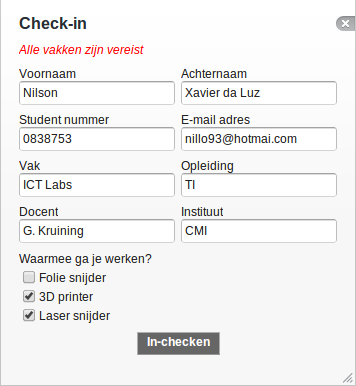
\includegraphics[width=175px, height=225px]{Images/checkin-student.png}
		\label{fig:checkin-student}
	}
	\subfigure[Checkin met errors]{
		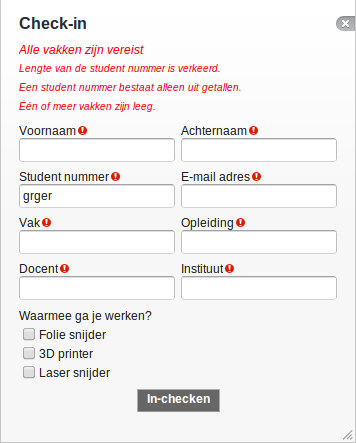
\includegraphics[width=175px, height=225px]{Images/checkin-student-error.png}
		\label{fig:checkin-student-error}
	}
	\caption{Checkin voor studenten}
\end{figure}

\subsection{Bedrijf en Overige}

Als een bedrijf of overige iemand in wilt checken dat krijgt diegene ook een eigen venster te zien. Hier wordt andere soort informatie gevraagd dat meer bij deze categorie past. Dit venster is te zien bij Figuur \ref{fig:checkin-company}. Ook hier wordt de ingevuld informatie gevalideerd om te zorgen dat alle informatie ingevuld is, dit is weergegeven in Figuur \ref{fig:checkin-company-error}. \\

\begin{figure}[Hh]
	\centering
	\subfigure[Checkin met ingevuld gegevens]{
		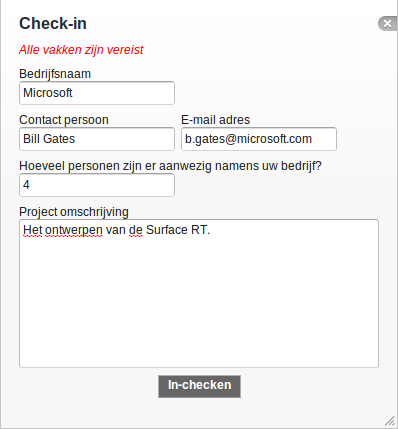
\includegraphics[width=175px, height=225px]{Images/checkin-company.png}
		\label{fig:checkin-company}
	}
	\subfigure[Checkin met errors]{
		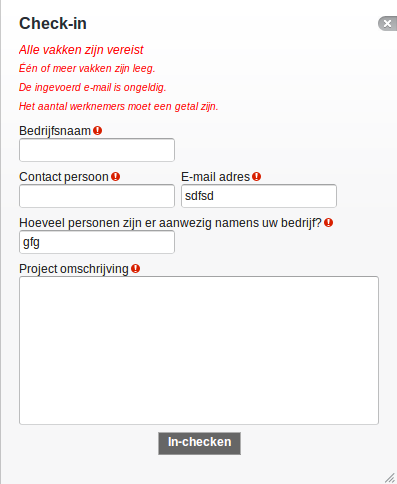
\includegraphics[width=175px, height=225px]{Images/checkin-company-error.png}
		\label{fig:checkin-company-error}
	}
	\caption{Checkin voor bedrijven}
\end{figure}

Zodra de gebruiker heeft ingecheckt, dan is de gebruiker vrij om gebruik te maken van het lab. Er komt dan een nieuwe element in de checkouts tabel te staan met de informatie van de gebruiker en een knop om uit te checken. Dit is te zien in Figuur \ref{fig:checkout-table}. \\

\begin{figure}[Hh]
	\centering
	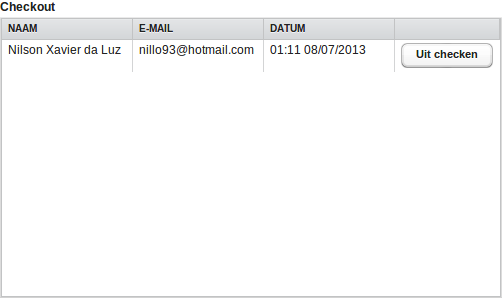
\includegraphics[width=0.65\textwidth]{Images/checkout-table.png}
	\caption{Pagina waar kan worden ingecheckt en uitgecheckt}
	\label{fig:checkout-table}
\end{figure}

\section{Checkout}

Wanneer de gebruiker klaar is en het lab wilt verlaten, wordt hij verzocht om eerste uit te checken. Dit gebeurt door zijn eigen informatie op te zoeken in de tabel en op de ``Uit checken'' knop te drukken. Er verschijnt dan een nieuwe venster om de benodigde informatie in te vullen over het project. Dit venster is weergegeven in Figuur \ref{fig:checkout-window}.

\begin{figure}[Hh]
	\centering
	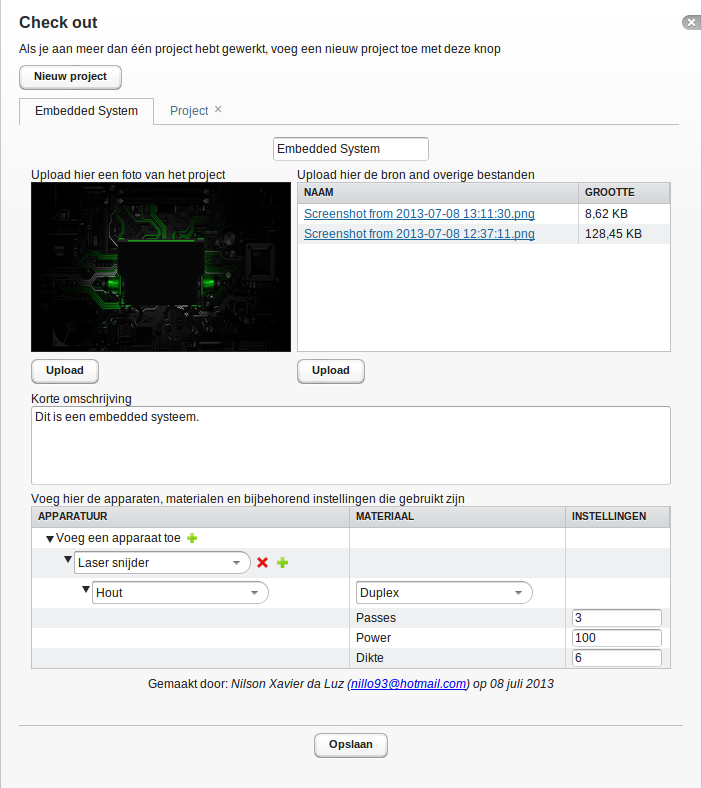
\includegraphics[width=0.65\textwidth]{Images/checkout-window.png}
	\caption{Venster waar kan worden uitgecheckt}
	\label{fig:checkout-window}
\end{figure}

Om te kunnen uitchecken wordt de volgende informatie gevraagd:

\subsection{Titel}

De titel wordt gebruikt om de project te identificeren. De titel moet uniek zijn.

\subsection{Foto}

Een foto van het project. Daarin moet duidelijk te zien zijn wat het project is.

\subsection{Bron bestanden}

Bron en overige bestanden van het project. Dit kan source code, 3D-modellen of iets anders zijn.

\subsection{Korte omschrijving}

Een korte omschrijving over wat het project is en/of doet.

\subsection{Instellingen}

Hier worden de gebruikte instellingen ingevuld van de gebruikte apparatten. Dit wordt gedaan door eerste apparaten toe te voegen, daarna materialen waaronder verschillende types te kiezen valt. Als een materiaal gekozen is, verschijnen de nodige instellingen van de gekozen apparaat en velden waar de instellingen kunnen worden ingevuld. \\

Er kunnen meerdere project worden aangemaakt voor het geval dat de gebruiker aan meerdere projecten heeft gewerkt. Dit wordt gedaan door op de ``Nieuw project'' knop bovenaan te drukken. Hierdoor wordt een nieuwe tab toegevoegd naast de tab van het bestaande project. \\
Als alles correct is ingevuld, dan wordt de checkout opgeslagen en is de gebruiker uitgecheckt.

\section{FabTool}

Het hoofdgedeelte van de webapplicatie is de FabTool, zie Figuur \ref{fig:fabtool}. Dit is waar projecten kunnen gezocht en bekeken, en waar beheerders overzicht kunnen houden over alle checkins en apparaten kunnen beheren.

\begin{figure}[Hh]
	\centering
	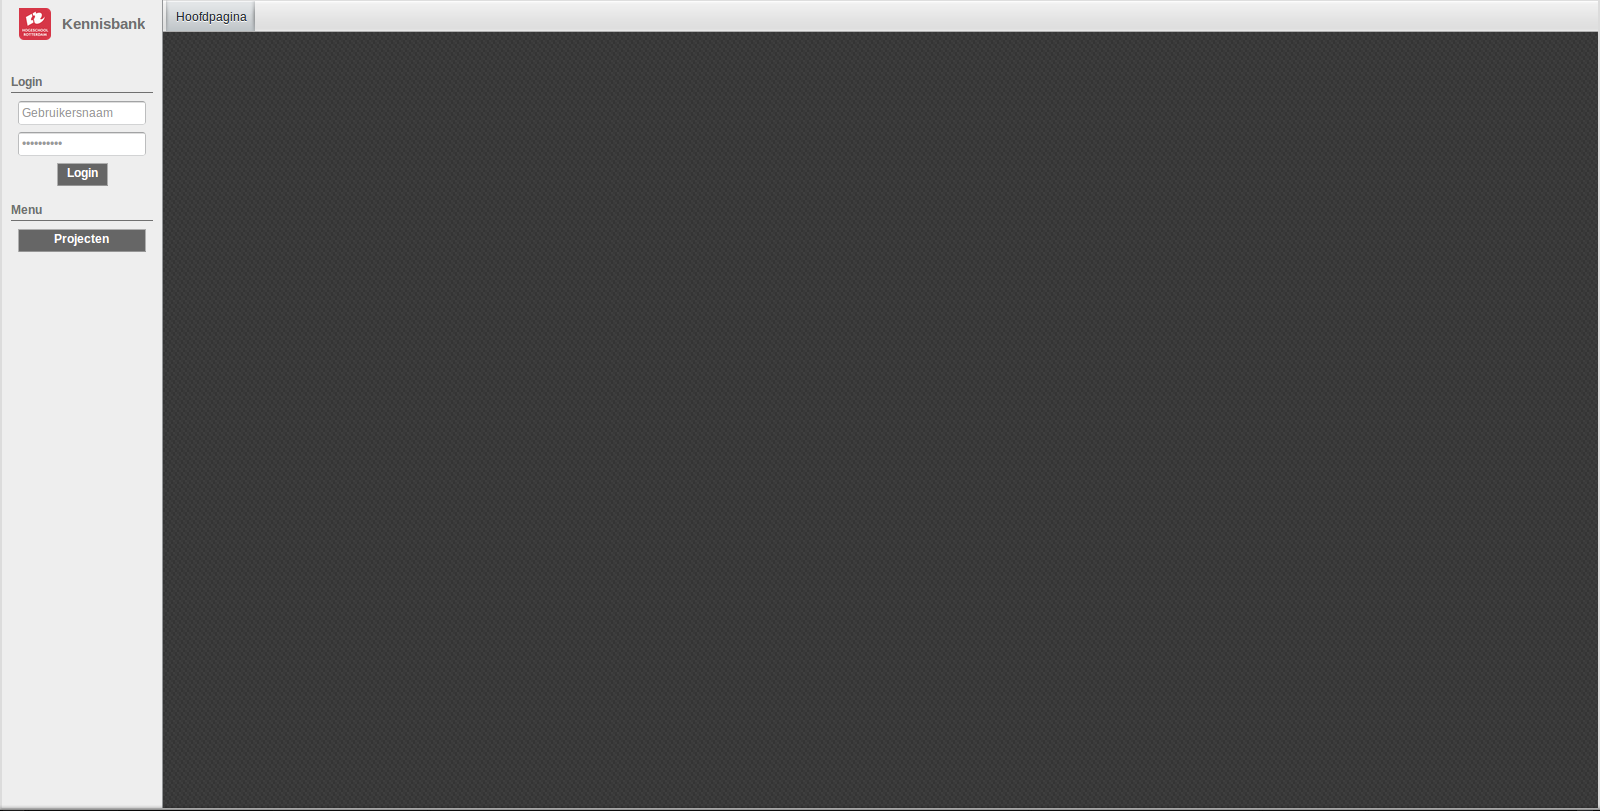
\includegraphics[width=1\textwidth]{Images/fabtool.png}
	\caption{Design van de FabTool}
	\label{fig:fabtool}
\end{figure}

\subsection{Projecten}

Een van de componenten van de FabTool zijn de projecten. Hier worden alle projecten die tot nu toe zijn gemaakt weergegeven, zoals het te zien is op Figuur \ref{fig:projects}.

\begin{figure}[Hh]
	\centering
	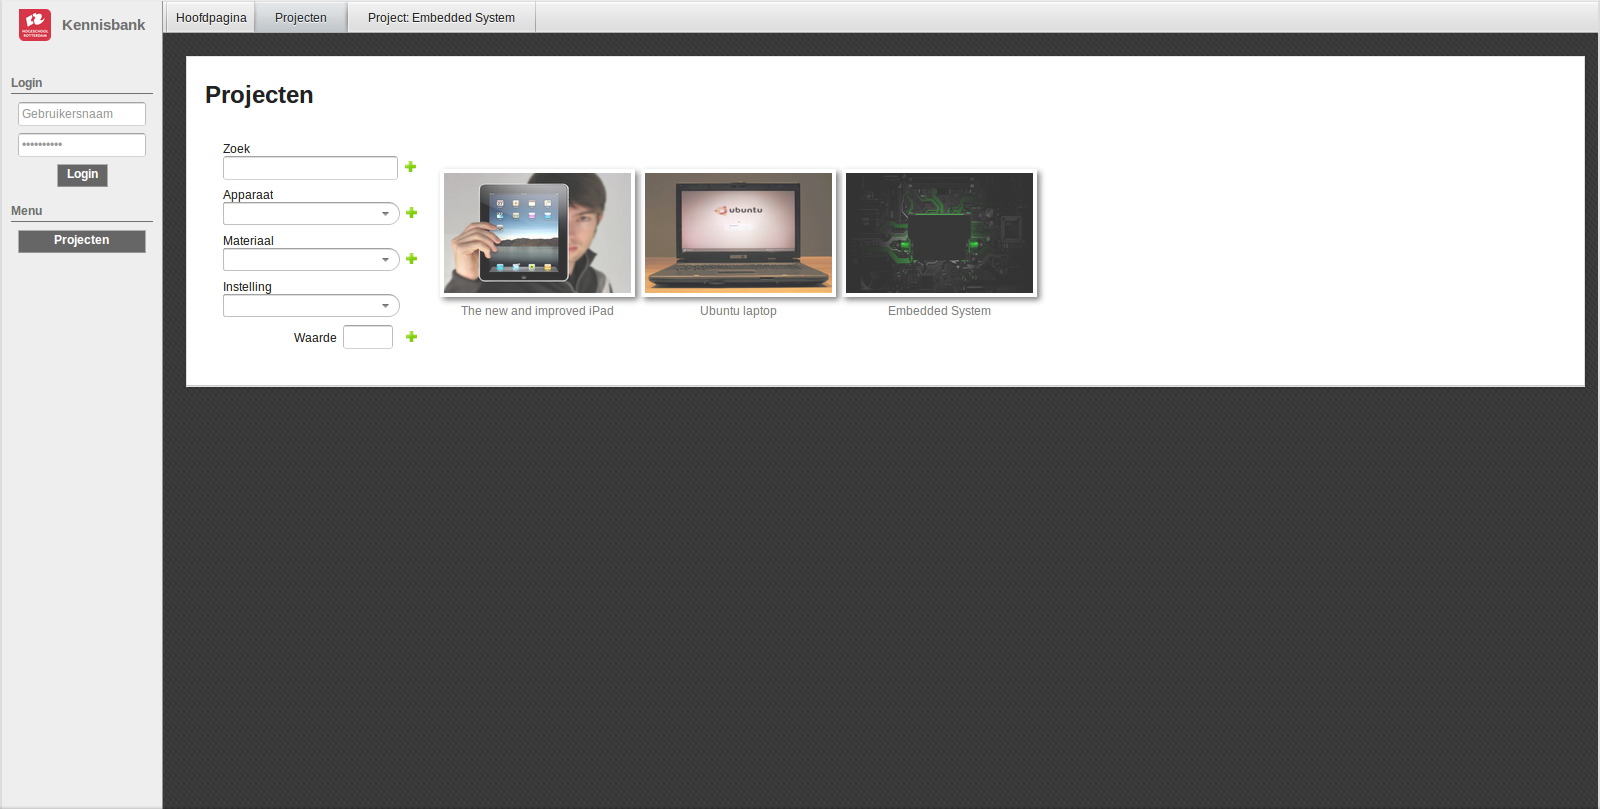
\includegraphics[width=1\textwidth]{Images/projects.png}
	\caption{Pagina waar projecten worden weergegeven}
	\label{fig:projects}
\end{figure}

Het geeft gebruikers ook de mogelijkheid om naar project te zoeken en te uit te filteren. Zoals het is weergegeven is in Figuur \ref{fig:filter-projects}, kunnen project op meerdere categori\"en worden gefilterd. Ze kunnen per soort apparaat, materiaal en instelling worden gezocht. Ook is het mogelijk om naar tekst te worden gezocht dat voorkomt in de titel of bij de omschrijving.

\begin{figure}[Hh]
	\centering
	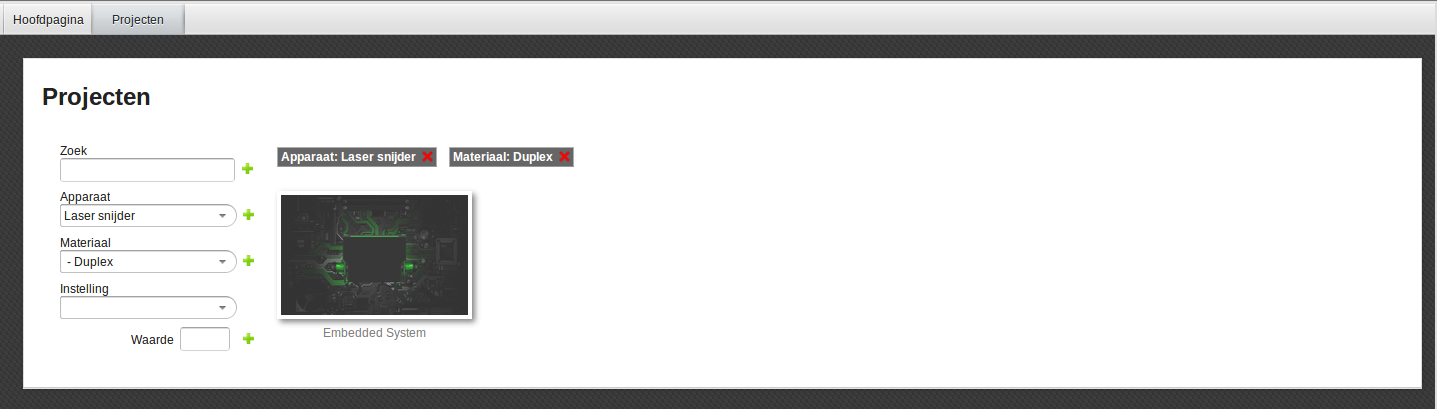
\includegraphics[width=1\textwidth]{Images/filter-projects.png}
	\caption{Projecten worden gefilterd}
	\label{fig:filter-projects}
\end{figure}

Als de gebruiker het project heeft gevonden waar hij naar zocht, kan hij erop klikken. Hierdoor verschijnt een nieuwe pagina met hetzelfde informatie dat tijdens het inchecken is ingevuld. Dit is te zien in Figuur \ref{fig:chosen-project}.

\begin{figure}[Hh]
	\centering
	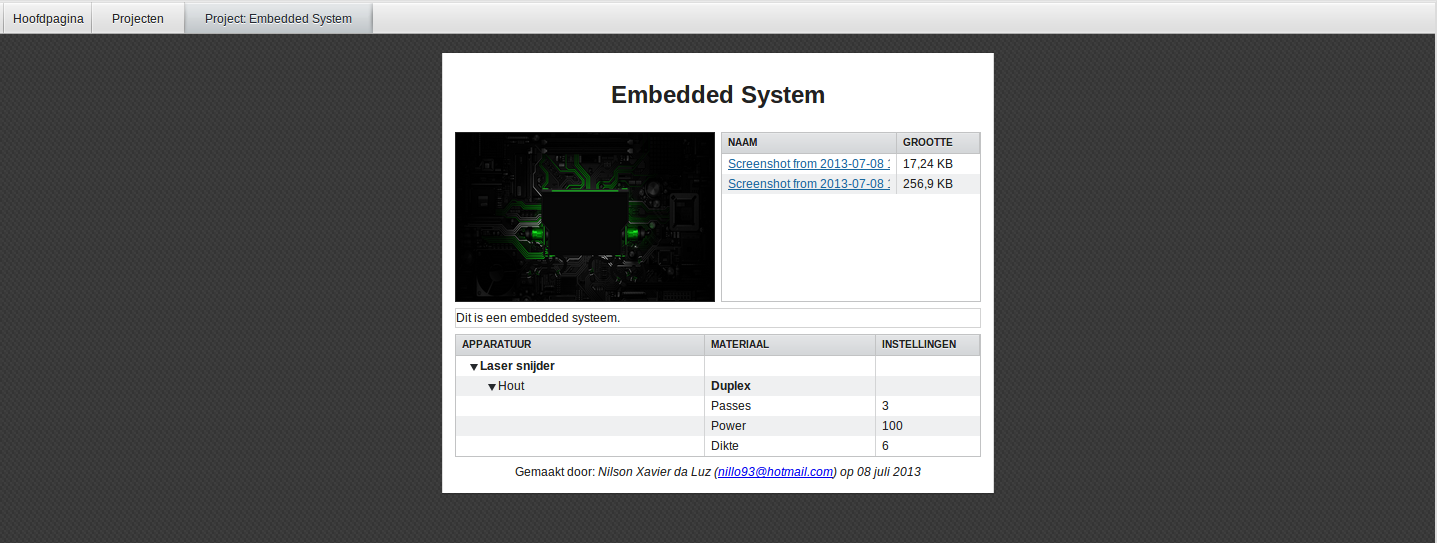
\includegraphics[width=1\textwidth]{Images/project.png}
	\caption{Gekozen project}
	\label{fig:chosen-project}
\end{figure}

\subsection{Administratie}
De Administratie is een pagina waar bijgehouden wordt wie er in de stadslab is geweest en wanneer. Dit wordt gedaan door een tabel weer te geven met alle check-ins en de mogelijkheid te geven om dezelfde check-ins te filteren, om hierdoor te kunnen zien in welke periode het druk was of juist rustig was.

\subsubsection{Table}

Om alle check-ins bij te houden hebben we een tabel toegevoegd aan de Administratie pagina. In deze tabel staan alle gegevens van de bijbehorende checkins. Deze tabel is te sorteren per soort gegeven.

\subsubsection{Timebuttons}

Voor het aanmaken van de zogenoemde timebuttons hebben we 3 verschillende concepten gemaakt.
\begin {itemize}
\item \textbf{Tabs}\\
Het eerste concept was om tabs toe te voegen in de Administratie pagina, die iedere keer een tabel had met nieuwe gegevens erin. Het aanmaken van een tabs bar was gelukt maar het uitvoeren ervan niet. De tabs functie is effectief voor het openen van een pagina classe, maar niet geschikt voor een panel die in de pagina is aangemaakt. 

\item \textbf{Menubar}\\
Het tweede concept was de menubar. Deze functie maakt buttons aan die ook nog een dropdown functie hebben. Het idee voor dropdown functie was om weeknummers of jaartallen te plaatsen, waardoor de tabel gefilterd kan worden. Het probleem aan deze aanpak is er een onduidelijke error ontstaat die we niet hebben kunnen oplossen en niet te veel tijd aan wilde besteden.

\item \textbf{Buttons}\\
De laatste en het definitieve concept is simpelweg het toevoegen van buttons. De timebuttons zijn verdeeld in 5 buttons ``Alle'', ``Vandaag'', ``Week'', ``Maand'' en ``Year''. Door alleen maar buttons toe te voegen kan er niet gefilterd worden. Daarom hebben we Date Selection functie toegevoegd.
\end {itemize}

\subsubsection{DateSelection}
Bij DateSelection hebben we twee PopupDatefields aangemaakt. Een StartDate en een Enddate. Als er gedrukt wordt op de pop-up button komt er een kalender tevoorschijn. Voor beide fields kan je handmatig de dagen kiezen, maar we wilden wat extra’s. 
We hebben een manier bedacht de Timebuttons effectief te maken, door de laatste periode te kiezen. Voor bijvoorbeeld de Timebutton ``week'' wordt de Enddate op de huidige dag geplaatst en de StartDate wordt doormiddel van de Enddate berekend zodat we de eerste dag van de week krijgen. Dit geldt ook voor jaar, maand of dag. 
Door de 2 dates datefields te gebruiken is het mogelijk de tabel te filteren.

\subsection{Aanpassingen}
In de aanpassingen pagina kan de apparaten, materialen, materiaal types en setting van een apparaat aangemaakt worden of al ze al in de database staan aangepast worden. Voor dit zijn er 2 tabellen aangemaakt de materialen tabel en de apparaten tabel.

\subsubsection{Materialentabel }
\begin{figure}[Hh]
	\centering
	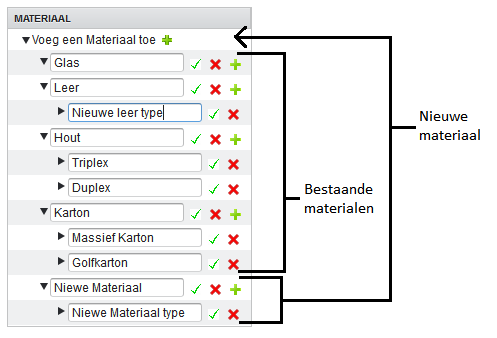
\includegraphics[width=0.5\textwidth]{Images/materiaaltable2.png}
	\caption{Materiaal tabel }
	\label{fig:materialentabel}
\end{figure}

In de tabel heb je de keuze om een nieuw materiaal toevoegen of bestaande materialen aan te passen. 

\begin {itemize}
\item \textbf{Nieuw materiaal}\\
Door op het plusje te drukken naast ``Voeg een Materiaal toe'' wordt er een textfield genaamd ''“Nieuwe Materiaal”'' toegevoegd aan de tabel. De ``Niewe Materiaal'' heeft 3 functies opslaan, verwijderen en het toevoegen van een materiaal type. Door een nieuw materiaal type toe te voegen ontstaat ``Niewe Materiaal type'', deze heeft de functies opslaan en verwijderen. Zie figuur \ref{fig:materialentabel}

\item \textbf{Bestaande materialen}\\
Alle materialen die zijn opgeslagen worden in de tabel weergegeven. Deze materialen kunnen worden aangepast door de 3 functies ernaast. Door een andere naam in te typen en het vinkje te drukken vervang je de benamingen van het bestaande materiaal. Het kruisje om het materiaal te verwijderen en het plusje om een nieuw type aan het materiaal toe te voegen. Voor een bestaand materiaal type hebben het vinkje en kruisje hetzelfde functie als het materiaal. Zie figuur \ref{fig:materialentabel}
\end {itemize}

\subsubsection{Apparatentabel }
\begin{figure}[Hh]
	\centering
	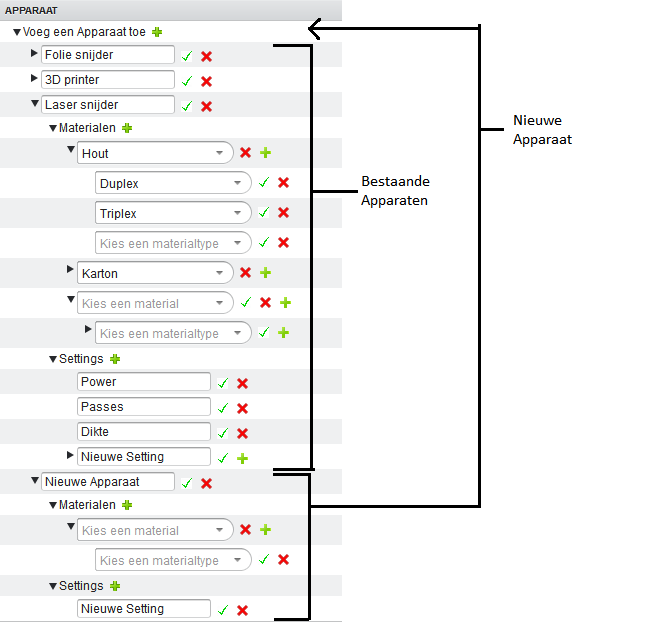
\includegraphics[width=0.5\textwidth]{Images/apparaattable2.png}
	\caption{Apparaten tabel }
	\label{fig:apparatentabel}
\end{figure}

De apparatentabel functioneert hetzelfde als de materialentabel. Het geeft je de keuze om een nieuw apparaat aan te maken of apparaten aan te passen.

\begin {itemize}
\item \textbf{Nieuw apparaat}\\
Om een nieuw apparaat volledig toe te voegen moet eerst een naam ervoor bedacht worden. Na het aan maken van het apparaat ontstaan er 2 kopjes, `` Materialen'' en `` Settings''. Het “ Materialen ``gedeelte'' is om bestaande materialen toegevoegd worden aan het apparaat. Dit is omdat sommige apparaten alleen functioneren met bepaalde materialen. Naast het toevoegen van bestaande materialen kunnen er ook materiaal types toegevoegd worden die verbonden met het materiaal die gekozen is. In het `` Settings'' gedeelte kan je zelf de instellingen van het apparaat intypen en toevoegen. Zie figuur \ref{fig:apparatentabel}

\item \textbf{Bestaande apparaten}\\
In de tabel staan alle apparaten die zijn toegevoegd met de bijhorende materialen, materiaal soorten en instellingen. Hier kan het apparaat en de bijhorende onderdelen aangepast of verwijderd worden. Zie figuur \ref{fig:apparatentabel}
\end {itemize}